%%% LaTeX Template: Two column article
%%%
%%% Source: http://www.howtotex.com/
%%% Feel free to distribute this template, but please keep to referal to http://www.howtotex.com/ here.
%%% Date: February 2011

%%% Preamble
\documentclass[	DIV=calc,%
							paper=a4,%
							fontsize=11pt%
							]{scrartcl}	 					% KOMA-article class

\usepackage{lipsum}													% Package to create dummy text

\usepackage[french]{babel}										% English language/hyphenation
\usepackage[protrusion=true,expansion=true]{microtype}				% Better typography
\usepackage{amsmath,amsfonts,amsthm}					% Math packages
\usepackage[pdftex]{graphicx}									% Enable pdflatex
\usepackage[svgnames]{xcolor}									% Enabling colors by their 'svgnames'
\usepackage[hang, small,labelfont=bf,up,textfont=it,up]{caption}	% Custom captions under/above floats
\usepackage{epstopdf}												% Converts .eps to .pdf
\usepackage{subfig}													% Subfigures
\usepackage{booktabs}												% Nicer tables
\usepackage{fix-cm}													% Custom fontsizes
\usepackage[utf8]{inputenc}
\usepackage[rightcaption]{sidecap} 
\usepackage{graphicx} %package to manage images
\usepackage{listings}
\usepackage{color}
\usepackage{subfig}

\definecolor{mygreen}{rgb}{0,0.6,0}
\definecolor{mygray}{rgb}{0.5,0.5,0.5}
\definecolor{mymauve}{rgb}{0.58,0,0.82}

\lstdefinestyle{customc}{
  belowcaptionskip=1\baselineskip,
  breaklines=true,
  frame=L,
  xleftmargin=\parindent,
  language=C,
  showstringspaces=false,
  basicstyle=\footnotesize\ttfamily,
  keywordstyle=\bfseries\color{green!40!black},
  commentstyle=\itshape\color{purple!40!black},
  identifierstyle=\color{blue},
  stringstyle=\color{orange},
}

\lstdefinestyle{customasm}{
  belowcaptionskip=1\baselineskip,
  frame=L,
  xleftmargin=\parindent,
  language=[x86masm]Assembler,
  basicstyle=\footnotesize\ttfamily,
  commentstyle=\itshape\color{purple!40!black},
}

\lstset{escapechar=@,style=customc}

\lstset{ %
  language=C,
  backgroundcolor=\color{white},   % choose the background color; you must add \usepackage{color} or \usepackage{xcolor}
  basicstyle=\footnotesize,        % the size of the fonts that are used for the code
  breakatwhitespace=false,         % sets if automatic breaks should only happen at whitespace
  breaklines=true,                 % sets automatic line breaking
  captionpos=b,                    % sets the caption-position to bottom
  commentstyle=\color{mygreen},    % comment style
  deletekeywords={...},            % if you want to delete keywords from the given language
  escapeinside={\%*}{*)},          % if you want to add LaTeX within your code
  extendedchars=true,              % lets you use non-ASCII characters; for 8-bits encodings only, does not work with UTF-8
  frame=single,	                   % adds a frame around the code
  keepspaces=true,                 % keeps spaces in text, useful for keeping indentation of code (possibly needs columns=flexible)
  keywordstyle=\color{blue},       % keyword style
  language=Octave,                 % the language of the code
  otherkeywords={*,...},           % if you want to add more keywords to the set
  numbers=left,                    % where to put the line-numbers; possible values are (none, left, right)
  numbersep=5pt,                   % how far the line-numbers are from the code
  numberstyle=\tiny\color{mygray}, % the style that is used for the line-numbers
  rulecolor=\color{black},         % if not set, the frame-color may be changed on line-breaks within not-black text (e.g. comments (green here))
  showspaces=false,                % show spaces everywhere adding particular underscores; it overrides 'showstringspaces'
  showstringspaces=false,          % underline spaces within strings only
  showtabs=false,                  % show tabs within strings adding particular underscores
  stepnumber=2,                    % the step between two line-numbers. If it's 1, each line will be numbered
  stringstyle=\color{mymauve},     % string literal style
  tabsize=2,	                   % sets default tabsize to 2 spaces
  title=\lstname                   % show the filename of files included with \lstinputlisting; also try caption instead of title
}



%%% Custom sectioning (sectsty package)
\usepackage{sectsty}													% Custom sectioning (see below)
\allsectionsfont{%															% Change font of al section commands
	\usefont{OT1}{phv}{b}{n}%										% bch-b-n: CharterBT-Bold font
	}

\sectionfont{%																% Change font of \section command
	\usefont{OT1}{phv}{b}{n}%										% bch-b-n: CharterBT-Bold font
	}



%%% Headers and footers
\usepackage{fancyhdr}												% Needed to define custom headers/footers
	\pagestyle{fancy}														% Enabling the custom headers/footers
\usepackage{lastpage}	

% Header (empty)
\lhead{}
\chead{}
\rhead{}
% Footer (you may change this to your own needs)
\lfoot{\footnotesize \texttt{Thibaut EHLINGER, Benjamin HERB} \textbullet ~Systèmes distribués et grilles : TP2}
\cfoot{}
\rfoot{\footnotesize page \thepage\ of \pageref{LastPage}}	% "Page 1 of 2"
\renewcommand{\headrulewidth}{0.0pt}
\renewcommand{\footrulewidth}{0.4pt}



%%% Creating an initial of the very first character of the content
\usepackage{lettrine}
\newcommand{\initial}[1]{%
     \lettrine[lines=3,lhang=0.3,nindent=0em]{
     				\color{DarkGoldenrod}
     				{\textsf{#1}}}{}}



%%% Title, author and date metadata
\usepackage{titling}															% For custom titles

\newcommand{\HorRule}{\color{DarkGoldenrod}%			% Creating a horizontal rule
									  	\rule{\linewidth}{1pt}%
										}
										
										\renewcommand\thesubsubsection{}

\pretitle{\vspace{-15pt} \begin{flushleft} \HorRule 
				\fontsize{15}{15} \usefont{OT1}{phv}{b}{n} \color{DarkRed} \selectfont 
				}
\title{Systèmes distribués et grilles : TP CUDA}					% Title of your article goes here
\posttitle{\par\end{flushleft}\vskip 0.1em}

\preauthor{\begin{flushleft}
					\large \lineskip 0.1em \usefont{OT1}{phv}{b}{sl} \color{DarkRed}}
\author{Thibaut EHLINGER, Benjamin HERB }											% Author name goes here
\postauthor{\footnotesize \usefont{OT1}{phv}{m}{sl} \color{Black} 
					Université de Strasbourg 								% Institution of author
					\par\end{flushleft}\HorRule}

\date{3 octobre 2016}																			



%%% Begin document
\begin{document}
\maketitle
\thispagestyle{fancy} 			% Enabling the custom headers/footers for the first page 
% The first character should be within \initial{}
\initial{D}\textbf{ans} ce TP nous devions exécuter des produits matriciels, qui sont des opérations mathématiques très gourmandes, avec des complexité algorithmique de l'ordre de $ \mathcal{O}(n^3)$. Afin de mettre pleinement à disposition les capacités de nos machines, nous avons donc exécuté les calculs cette fois sur la carte graphique de nos ordinateurs, grâce à la technologie CUDA (Compute Unified Device Architecture). Comme pour le TP précédent, il s'agit d'un produit de matrices $ 4096 \times 4096$. Il est à noter que sur les cartes graphiques des machines de la salle J4 , des \textbf{gtx680, architecture Kepler}, nous n'avions pas le droit de lancer des calculs trop longs. Pour des raisons de sécurité, sans doute, il nous était impossible de réaliser des calculs dépassant les 11-12 secondes. Néanmoins cela ne nous a pas empêché d'obtenir des résultats concluants, étant donné que de toute manière nous cherchions à optimiser le temps de calcul.\par
Dans ce rapport, nous expliquerons tout d'abord les problématiques de dimensionnement des blocs de \textit{threads} et leurs conséquences. Puis, nous étudierons les différents temps et puissances de calculs obtenus en fonction du dimensionnement des blocs, sur le kernel 2. Enfin, nous traiterons les expérimentations effectuées sur le kernel 4, en nous concentrant sur la mémoire partagée : comment l'utiliser au mieux et les bienfaits de son utilisation. 

\section{Contexte}
\subsection{Environnement d'expérimentation}
Comme dit précédemment, nous travaillons ici sur une carte graphique \textbf{gtx680, architecture Kepler}. Les données ont été prélevées une seule fois, puis notées sur un fichier \texttt{Excel} prévu à cet effet. Ensuite, nous avons converti ces donnés au format \texttt{csv}, qui ont ensuite été représentées graphiquement avec \texttt{Gnuplot}. Parallèlement, nous avons aussi intégré dans ce rapport un graphique qui était déjà généré dans la feuille \texttt{Excel}.
\subsection{Des dilemmes de pavage}
L'intérêt du calcul distribué sur une carte graphique est de mettre à profit la puissance de calcul d'une GPU. En revanche, les GPU sont optimisées pour les calculs dits \textit{SIMD}, pour \textit{single instruction - multiple data}, ce qui veut dire qu'il est très simple pour une carte graphique de réaliser moult fois la même instruction sur un grand jeu de données diversifiées. Le calcul matriciel correspond exactement à ce genre de calculs.\par
Une GPU s'organise en blocs de \textit{threads}, aussi appelés \textit{warps}. Chaque \textit{thread} est en charge d'une toute partie du calcul. En effet ces \textit{threads} ne sont pas faits pour se comporter comme des \textit{threads} POSIX : ils sont conçus pour réaliser des calculs très très simples. Ici, par exemple, un \textit{thread} est en charge d'une seule et unique case de la matrice résultat à la fois. Ce qui veut dire qu'il gère la somme de $Nb_{colonnes}(\mathcal{A}) \times (Nb_{lignes}\mathcal{B})$ produits de \texttt{double}.\par
Une première contrainte est que le nombre de \textit{threads} par bloc ne peut dépasser 1024. On est aussi limité pour le nombre total de blocs, mais cette limite ne nous a pas concerné pour notre TP, celle-ci allant de $2^{16}$ à $2^{31} - 1$. Le dilemme mis en exergue dans ce TP concerne le dimensionnement de ces blocs : en effet, on peut subdiviser les matrices à multiplier entre elles en blocs de différentes tailles, ce qui a différentes conséquences. Les questions auxquelles nous essaierons de répondre sont : 
\begin{itemize}
\item Sur une seule dimension, quelle semble être la largeur optimale?
\item Sur deux dimensions, quel(s) facteur(s) influe le plus sur les différentes puissances/durées de calcul?
\end{itemize}

\section{Allocation de blocs d'une seule dimension}
\begin{figure}
    \subfloat[Temps de calcul en fonction de la largeur de bloc.
      \label{img:1DK1_time}]{%
      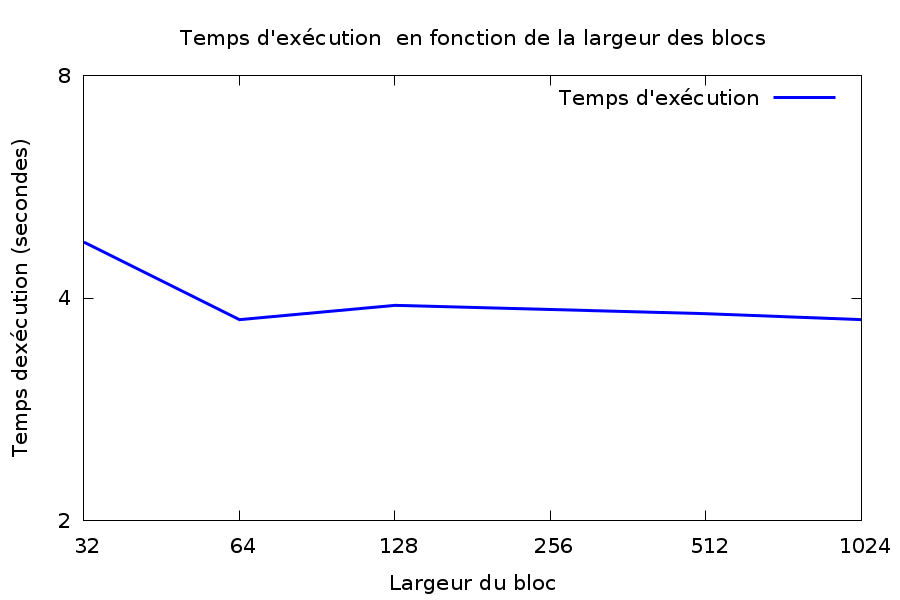
\includegraphics[keepaspectratio,width=0.47\textwidth]{img/bloc_1D_time.png}
    }
    \hfill
    \subfloat[Puissance de calcul en fonction de la largeur de bloc.
      \label{img:1DK1_power}]{%
      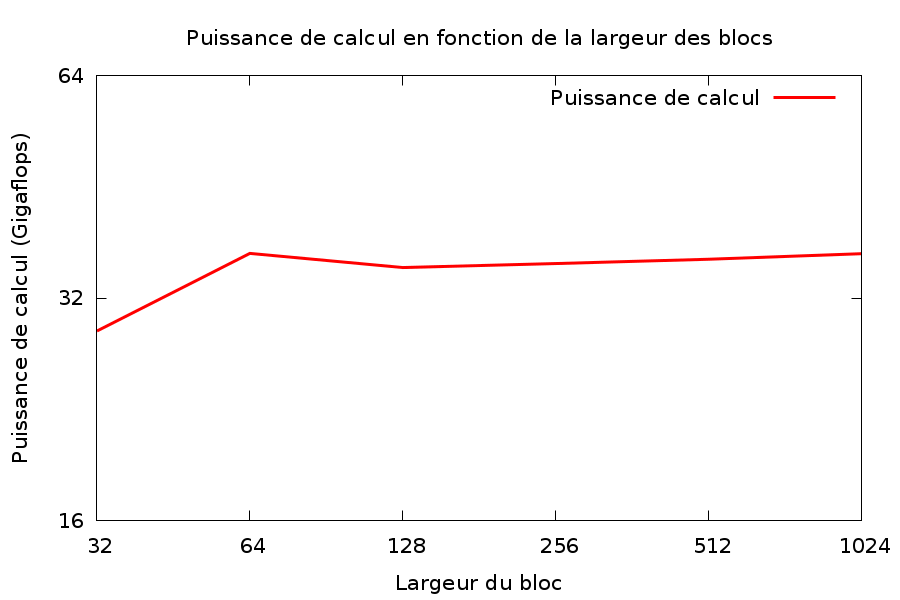
\includegraphics[keepaspectratio,width=0.47\textwidth]{img/bloc_1D_power.png}
    }
    \caption{Temps et puissance de calcul en fonction de la largeur du bloc 1D.}
    \label{fig:1DK1}
\end{figure}

\subsection{Analyse relative}
La figure \ref{fig:1DK1} présente, à gauche, le temps d'exécution du produit en fonction de la largeur du bloc, et à droite, la la puissance d'exécution en fonction de la largeur du bloc.\par
Dans l'étude \textbf{relative} des résultats, c'est à dire lorsqu'on les compare entre eux, deux choses importantes sont à notes : 
\begin{itemize}
\item Le seul écart notable est entre 32 et 64 \textit{threads} de largeur pour le bloc. Comme mentionné en cours, les meilleurs résultats sont souvent obtenus entre 32 et 64 threads par bloc, ici la bonne réponse est 64.
\item 64 n'est que légèrement meilleur que les valeurs qui lui sont supérieures. Néanmoins 64 est clairement la meilleure valeur. C'est le meilleur compromis entre le nombre de blocs et la taille des blocs. Au-delà, les blocs sont trop grands pour être le plus performant. En deçà de 64 \textit{threads}, il y a sûrement trop de communication de données par rapport au temps total de calcul.
\end{itemize}

\subsection{Analyse absolue}
Dans l'absolu, ce produit matriciel avec un bloc 1D n'est pas très performant. En effet, pour comparaison, le même calcul avec le CPU a pris \textbf{3.73 secondes} pour une puissance de calcul de \textbf{36.81 gigaflops}. On voit donc que le CPU est plus performant que le GPU en bloc 1D. On comprend donc que la GPU n'est pas suffisamment monopolisée, le calcul pas assez bien distribué pour qu'il puisse être réellement rentable.

\section{Allocations de blocs 2 dimensions sans mémoire partagée}
Dans cette partie, nous allons donc jouer sur un deuxième facteur pour améliorer les performances et les rendre enfin meilleures que sur la CPU. Pour ce faire, nous allons désormais jouer sur \textbf{deux} paramètres afin d'étudier les résultats : la \textit{hauteur} et la \textit{largeur} des blocs. Ainsi, les blocs pourront potentiellement contenir des données en mémoire de manière plus contiguë. Cela pourrait potentiellement diminuer le temps de calcul étant donné que les mêmes données seront peut-être chargées en cache pour plusieurs \textit{threads}.\par
La figure \ref{img:2DK2_power} est une représentation des résultats obtenus. Comme il s'agit d'un tableau à trois dimensions, le graphe utilisé ici, qui nous a gracieusement été fourni par notre enseignant, se sert de l'axe des abscisses pour la variable $\mathcal{X}$, la largeur du bloc, et de l'axe des ordonnées pour la variable $\mathcal{Y}$.
\begin{figure}
      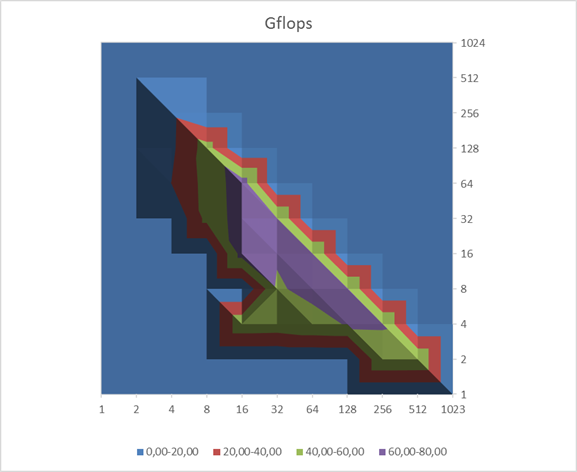
\includegraphics[keepaspectratio,width=12cm]{img/Gflops_depending_bloc_size.png}
      \label{img:2DK2_power}
	  \caption{Puissance de calcul en fonction de la hauteur du bloc Y (en ordonnées) et de la largeur des blocs X (en abscisse).}
\end{figure} 

\section{Annexe : code}

\subsection*{Initialisation MPI}
\begin{lstlisting}
#include <stdio.h>
#define N 10

/* Initialisation of processor coordinates */

void ProcessorInit(void){
	MPI_Comm_size(MPI_COMM_WORLD,&NbPE);
  	MPI_Comm_rank(MPI_COMM_WORLD,&Me);
}
\end{lstlisting}

\newpage

\subsection*{Calcul de l'offset pour un processus {\texttt{Me} donné}}
\begin{lstlisting}
/* Compute the current step offset, in the MPI program, to access right C lines */ OffsetStepLigC = ((Me + step) * LOCAL_SIZE) % SIZE; 
\end{lstlisting}

\subsection*{Boucle principale}
\begin{lstlisting}
void ComputationAndCirculation()
{
 unsigned long step;
 
 for(step=0;step<NbPE;step++) { 
  OneLocalProduct(step);
  OneStepCirculation(step);
 }
}
/* Elementary circulation of A and B.                                            */
void OneStepCirculation(unsigned long step)
{
 MPI_Status   status;

 MPI_Sendrecv_replace(A_Slice, SIZE*LOCAL_SIZE, MPI_DOUBLE, (Me-1+NbPE)%NbPE, 0, (Me+1)%NbPE, 0, MPI_COMM_WORLD, &status);
}


\end{lstlisting} 
\end{document}